\documentclass[11pt]{report}
\usepackage[utf8]{inputenc}

% Line
\newcommand{\HRule}{\rule{\linewidth}{0.5mm}}

% Tweak texcount
%TC:group comment 0 0
%TC:macro \plan 0
%TC:macro \gavin 0
%TC:macro \question 0
%TC:macro \insertref 0
%TC:macro \todo 0
%TC:macro \question 0
%TC:macro \lstinline [xx]
%TC:macro \inlinephp [xx]
%TC:envir lstlisting [] xall
%TC:envir comment 0 0

% pictures!
\usepackage{graphicx}
\graphicspath{ {images/} }

% sub figures
\usepackage{caption}
\usepackage{subcaption}

% counts how many pages there are
\usepackage{lastpage}

% indent
% \usepackage{indentfirst}

% cross referencing

% Nicer tables
\usepackage{booktabs}

% Reference in harvard
\usepackage[style=ieee,doi=true,url=true,backend=bibtex]{biblatex}
\addbibresource{references.bib}

% maths
\usepackage{amsmath}

% custom float settings
\usepackage{float}

% \begin{verbatim} literal text
\usepackage{verbatim}

% adjust header/footer
\usepackage{fancyhdr}
\pagestyle{fancy}

% URL's
\usepackage{hyperref}
\usepackage{breakurl}

% Appendix
\usepackage[page, titletoc]{appendix}

% Glossery
\usepackage{glossaries} % [toc,section=section]
\makeglossaries

% Todos's \todo, \listoftodos, \missingfigure
\usepackage[textwidth=4cm]{todonotes} % disable option disables notes
\setlength{\marginparwidth}{4cm} %wider margin

% insert ref's
\newcommand{\insertref}[1]{\todo[inline,color=green!40]{#1}}

% gavin notes
\newcommand{\gavin}[1]{\todo[color=green!40]{\textbf{G:}~#1}}

% lorna's notes
\newcommand{\lorna}[1]{\todo[color=purple!40]{\textbf{L:}~#1}}

% Plan notes
\newcounter{plancount}
\newcommand{\plan}[1]{%
    \refstepcounter{plancount}%
    \todo[inline,color=yellow!40]{\textbf{P\theplancount:}~#1}%
}

% Question in margin
\newcounter{questioncount}
\newcommand{\question}[1]{%
    \refstepcounter{questioncount}%
    \todo[color=pink!40]{\textbf{Q\thequestioncount:}~#1}%
}

% Commas
\usepackage[group-separator={,}]{siunitx}

% Color
\usepackage{xcolor}
\usepackage{textcomp}

% Code
\usepackage{listings}
\newcommand*{\inlinesql}{\lstinline[language=SQL]}
\newcommand*{\inlinehtml}{\lstinline[language=HTML]}
\newcommand*{\inlinephp}{\lstinline[language=PHP]}
\newcommand*{\inlinetext}{\lstinline[language=textwithspaces]}

% Colors
\definecolor{string}{HTML}{DD0000}
\definecolor{comment}{HTML}{FF8000}
\definecolor{keyword}{HTML}{007700}
\definecolor{default}{HTML}{0000BB}

% PHP code style
\lstdefinestyle{phpcolor}{
  language        = php,
  basicstyle      = \footnotesize\ttfamily,
  keywordstyle    = \color{keyword},
  stringstyle     = \color{string},
  identifierstyle = \color{default},
  commentstyle    = \color{comment},
  emph            =[1]{php},
  emphstyle       =[1]\color{red},
  emph            =[2]{if,and,or,else},
  emphstyle       =[2]\color{keyword},
  breaklines=true,
  upquote=true,
  tabsize=2,
  showspaces=false
}

\lstdefinestyle{showspaces}{
  basicstyle      = \footnotesize\ttfamily,
  breaklines=true,
  upquote=true,
  showstringspaces=true,
  showspaces=true
}

\lstdefinelanguage{textwithspaces}{
    alsoletter={0,1,2,3,4,5,6,7,8,9,.,/,:},
    showstringspaces=true,
    style=showspaces,
    morestring=[b]|
}

\colorlet{punct}{red!60!black}
\definecolor{delim}{RGB}{20,105,176}
\colorlet{numb}{magenta!60!black}

\lstdefinelanguage{json}{
    basicstyle=\footnotesize\ttfamily,
    showstringspaces=false,
    breaklines=true,
    showspaces=false,
    literate=
     *{0}{{{\color{numb}0}}}{1}
      {1}{{{\color{numb}1}}}{1}
      {2}{{{\color{numb}2}}}{1}
      {3}{{{\color{numb}3}}}{1}
      {4}{{{\color{numb}4}}}{1}
      {5}{{{\color{numb}5}}}{1}
      {6}{{{\color{numb}6}}}{1}
      {7}{{{\color{numb}7}}}{1}
      {8}{{{\color{numb}8}}}{1}
      {9}{{{\color{numb}9}}}{1}
      {:}{{{\color{punct}{:}}}}{1}
      {,}{{{\color{punct}{,}}}}{1}
      {\{}{{{\color{delim}{\{}}}}{1}
      {\}}{{{\color{delim}{\}}}}}{1}
      {[}{{{\color{delim}{[}}}}{1}
      {]}{{{\color{delim}{]}}}}{1},
}

% Graphics
\usepackage{tikz}
\usetikzlibrary{automata,chains}

% header and footer
\rfoot{\thepage\ of \pageref{LastPage}}
\cfoot{}
\lfoot{}

% Use wide margins, but not quite so wide as fullpage.sty
%\marginparwidth 0.5in 
%\oddsidemargin 0.25in 
%\evensidemargin 0.25in 
%\marginparsep 0.25in
%\topmargin 0.25in 
%\textwidth 6in \textheight 8 in

\begin{document}
% title and thanks
\begin{titlepage}
\begin{center}

\textsc{\LARGE University of Manchester}\\[1.5cm]
\textsc{\Large School of Computer Science\\Project Report 2014}\\[0.5cm]

% Title
\HRule \\[0.4cm]
{ \huge \bfseries Using Machine Learning to predict personal expenditure \\[0.4cm] }

\HRule \\[1.5cm]

% Author and supervisor
\begin{minipage}{0.4\textwidth}
\begin{flushleft} \large
\emph{Author:}\\
Pez \textsc{Cuckow}
\end{flushleft}
\end{minipage}
\begin{minipage}{0.4\textwidth}
\begin{flushright} \large
\emph{Supervisor:} \\
Gavin \textsc{Brown}
\end{flushright}
\end{minipage}

\vfill

% Bottom of the page
%{\large \today}

\end{center}
\end{titlepage}
%TC:ignore
\begin{abstract}
Abstract pending
\plan{Abstract, assuming I need one}


\par\noindent{\small{\bf Keywords:} MY KEYWORDS, GO HERE}

\end{abstract}
%TC:endignore

%\clearpage
\vspace*{1.4in}
\begin{center}
  {\textbf{Acknowledgements}} \\
\end{center}
\begin{quotation}
  Thanks everyone, y'all great.
\end{quotation}

% define words
\newglossaryentry{transactor}
{
  name={transactor},
  description={somewhere money is spent, e.g. Tesco, Sainsbury's, Byte Cafe.}
}

\newglossaryentry{transaction}
{
  name={transaction},
  description={a single movement of money from/to a Transactor}
}

\newglossaryentry{category}
{
  name={category},
  description={transactors have a category and a subcategory, e.g. Tesco = Shopping, Groceries}
}

\newglossaryentry{reference}
{
  name={reference},
  description={the memo or message that is included on the bank statement with a transaction}
}

\newglossaryentry{mapping}
{
  name={mapping},
  description={this connects the reference found on a statement to a Transactor. e.g. Snbs, Sains => Sainsbury's}
}

\newglossaryentry{globaltransactor}
{
  name={global transactor},
  description={the system holds two collections of transactors and mapping's, the global ones
are shared between all users, and only accessed with the admin panel.}
}

\newglossaryentry{usertransactor}
{
  name={user transactor},
  description={unique to each user}
}

% start of document
\tableofcontents
\listoffigures
\listoftables
\printglossaries

\clearpage

% Password entropy & security
% Personalised model from Five models detail, per catecory, per person
% Hypothesise one models

% start of writing
\chapter{Introduction}

\begin{comment}
This chapter puts the work into context. Having read it, the reader should be left in no doubt as to:

- the topic area to which the work applies
- why the work is being done
- what else has been done in the area and by whom
 - how the author proposes to tackle the problem: The project proposal is often expressed in terms of a main objective and possibly one or more additional objectives. It is useful to define "milestones" or "sub-goals" that mark the progress towards the objectives. 
 - It is common to end this chapter with a brief overview of each of the subsequent chapters of the report.
\end{comment}

Traditionally the management of personal finances is performed by viewing bank statements provided by the users bank, however, even in this modern age of 'internet banking' banks offer a limited set of tooks that mimic the paper statements that would have been sent in the past.

This project sets out to build an online application that can be used to manage personal finances. There are two main parts of the project; firstly Users can upload  bank statements, which are displayed and navigated in an intuitive manner; secondly, once the application has enough historical data, predicting the users future outflow.

\section{Motivation}
% \plan{Help make managing finances easier, basic survey of people + appendix with details, any relevant paperts}
There are four main steps when producing and using a budget, recording previous expenses, sorting these into categories
using this historical information to guess future expenditure and evaluate accuracy of these predictions and using new information to update them.

Since the liquidity crisis of 2009 \cite{gore2010}, budgets have been squeezed and the average persons personal disposable income has fallen, hitting a nine-year low in 2012\cite{barnard2012households}. With experts suggesting that ``Budgets are essential for financial planning''\cite{wsj2013budget}, research suggesting that personal budgets lead to a ``positive impact on ``mental wellbeing''\cite{tlap2013budget} and guides from UCAS, the UoM SU Advice Centre and The Manchester University Crucial Guide encouraging use of budgeting, it is clear that producing a budget is of benefit.

However, in an informal survey\footnote{Appendix \ref{app:budgetsurvey}} the majority of students surveyed, did not make a budget. An easier way to produce a budget can hopefully increase the amount of students relying on one.

Increasing use of debit cards\cite{bbc2010debit} means that bank statements contain more and more information about where people spend their money. With access to those bank statements now provided online, with most UK banks offering the option to export \gls{transaction} history, individual users can collate a database of their personal spending habits.

The increasing availability of this data, combined with more detailed transaction history makes it possible to automate the four main steps of producing a budget, and this is the idea behind the project.

\section{Existing work in this area}

\subsection{Management}
There are several other applications implement management features found in this project, most notably Lloyds TSB Money Manager \cite{lloyds2014money}, which was the first money management application provided by a UK bank.

The service is available to Lloyds TSB current account holders as part of their online banking and offers several key features, however all of the features revolve around documenting historical spending.

\begin{list}
\item Categorising spending
\item Creating spending plans per category.
%\item View dates money came in and out in a calendar
\item Viewing money spent per category
\item Track progress of budget targets
\end{list}

\begin{figure}[h]
    \centering
    \includegraphics{moneymanager}
    \caption{Spending Analysis on Money Manager \citet{lloyds2014money}}
    \label{fig:moneymanager}
\end{figure}

Mint.com is a US only personal finance service that provides features similar to those provided by LLoyds. They include 


\section{Aims and Objectives}
\plan{Things I set out to do, designed by talking to people to get an idea of features they would like}

\subsection{Parsing Statements}
\plan{Loading a statement into the actual system, do I mention named entity resolution here?}

\subsection{Predicting expenditure}
\plan{Predicting how much money you're going to spend in the future (or next month)}

\section{Overview of Report}
\plan{This report covers some of the key design decisions, implementation decisions and then what the application does}

\chapter{Background}
\label{cha:background}

\begin{comment}
Chapter 2: Background and literature survey
This chapter should give essential background information with references to published material in research papers, books, URLs, magazine articles and even newspapers. Expand on any references to other work that have been mentioned in Chapter 1. Refer to the notes on references (below) for the preferred way of referencing publications. The reader, stimulated by the presentation of ideas in this section, may be led to consult some or all of the referenced publications. This section will be useful for any student in a subsequent year who wishes to take the project further.
\end{comment}

As outlined in Chapter \ref{cha:introduction} the project consists of two major parts: a financial management service, which can be used to view historical spending and gain understanding of personal finances; and a forecasting element which predicts how much spending will occur in the future. 
\question{Include this?} \question{Technically it's spending or receiving "transaction" but this becomes very wordy?}

\section{Statement Management}
There are existing applications that implement similar features to the money management aims of this project\question{Mention the current "bad" internet banking here?}, most notably Lloyds TSB Money Manager, the first and only personal money management application provided by a UK bank and Mint.com a United States (US) only personal finance service \parencite{lloyds2014moneymanager, mint2014whatismint}.

\subsection{Lloyds Money Manager}
The service is available to Lloyds TSB current account holders as part of their online banking and it's features revolve around documenting historical spending \parencite{lloyds2014money}.

The key features include:
\begin{itemize}
\item Categorising spending
\item Creating spending plans per category
%\item View dates money came in and out in a calendar
\item Viewing money spent per category
\item Track progress of budget targets
\end{itemize}

Customer reviews of the service highlight the usefulness of spending analysis screen, which includes a breakdown of spending in each \gls{category} (Fig. \ref{fig:moneymanager}, as well as the spending calendar, which displays money spent in a day by day format.
%
The reviews, however, also highlight some shortcomings, noting that changes to categories are not reflected immediately, categories are often incorrect and that it's not possible to override the \gls{category} for a single transaction, for example food bought at a petrol station is placed in the Car \gls{category} and cannot be moved \cite{moneywatch2011lloyds, moneysupermarket2011lloyds}.

\begin{figure}[h]
    \centering
    \includegraphics{background/moneymanagerchart}
    \caption{Spending Analysis by category on Money Manager \parencite{lloyds2014money}}
    \label{fig:moneymanager}
\end{figure}

A key advantage of the money manager is that Lloyds already have access to their customer data, so there is no data entry or upload required, which could be confusing and off-putting to potential users.

\subsection{Mint.com}
Mint.com offers very similar features to LLoyds but it limited to the US. However, Mint automatically logs into the users online bank account and downloads their statements authenticating with their banking username and password. It's reported that this feature relies on the use of application programming interface's (API) at each bank which Intuit (the company behind Mint) have negotiated access individually, though Intuit have published no information to support or dispute this \cite{stackoverflow2012bankingapi, stackoverflow2012bankingapi2}.
% 
Although this feature is clearly useful and saves time for the users, it does make Mint responsible for storing their customers Internet banking passwords and presumably involves fee payments to the banks providing these API's. \question{Should I have more detail on what mint/lloyds do?}
%
For these reasons it was decided that automatic statement uploading was outside of the budget and scope of this project, however, the project should support manual upload of statements to avoid date entry of users. \question{Does this need backing up?}

\subsection{Mobile Apps}
Mobile applications or `apps' as they are commonly known have seen a surge in popularity since the release of startphones and are a common target for small pieces of software, such as financial organisation \parencite{purcell2011half}.

The three most popular iPhone personal financial applications \cite{itunes2013topapps}, at the time of planning the project, all offered features very similar to those found in the Lloyds Money Manager and Mint. The most popular features being grouping money by \gls{category} and graphs of spending history.
% 
However, they all had the same drawback, the user had to manually enter all of their transactions and set categories for them, which appears time consuming and error prone, particularly on a mobile app \cite{spendee2014spendee,budgt2013budgt,bluetags2014pocket}.

The increase of mobile usage should be considered when planning the features of the project, with the project ensuring mobile compatibility and if possible, avoiding manual data entry. \plan{This needs improving}

\section{Prediction}
%\plan{Ways other people try to predict the future expenditure (in stocks etc...)}

There are various approaches to making predictions of financial spending, each with their own advantages and disadvantages \question{Not sure if this is relevant}. Predicting future transactions before they occur is technically similar to the work done by investors on the stock market, where the objective is to predict whether the value of a stock will fall or increase in order to make buy/sell decisions.

Preifer and Carraway demonstrated that Markov Chain Models can be used to model customer relationships with a business and predict the expected value of a marketing engagement with an individual customer. By creating a transition matrix of a particular customer transitioning from not spending to spending and visa versa over five periods\footnote{An `illustration' assuming a customer will never return after 5 months of not spending}, they were able to estimate the likely-hood of a spend occurring in a given period, Fig. \ref{fig:preifermarkovchain} shows a graphical representation of the model that was produced, the states represent the five periods, where $p_{i}$ is the probability of the transition occurring during period $i$ \cite{pfeifer2000modeling}.
% 
The paper is able to calculate the expected loan to value ratio (LTV) for the customer over the periods, by taking a matrix costs and gains associated with a purchase in each period and multiplying that by the probability of a purchase occurring taken from the transition matrix. This gives the expected present value for each period, which can be used to decide when to end a relationship with a customer (preventing the costs).
%
They demonstrate applying Markov Chain Models to a larger dataset, calculating the optimal policy for ending relationships with customers depending on varying costs concluding that the use of MCM's is an effective way of making customer relationship decisions. However, this paper assumes the company performing these predictions already knows how much money a customer will spent during each interactions and is focussed around calculating the probability of a spend occurring. An implementation applied to the personal spending space will require a way to predict the value of the future transaction.
\question{Mention what HMM's are here?}

\begin{figure}[h]
    \centering
    %\includegraphics[width=\textwidth]{background/markovchain}
    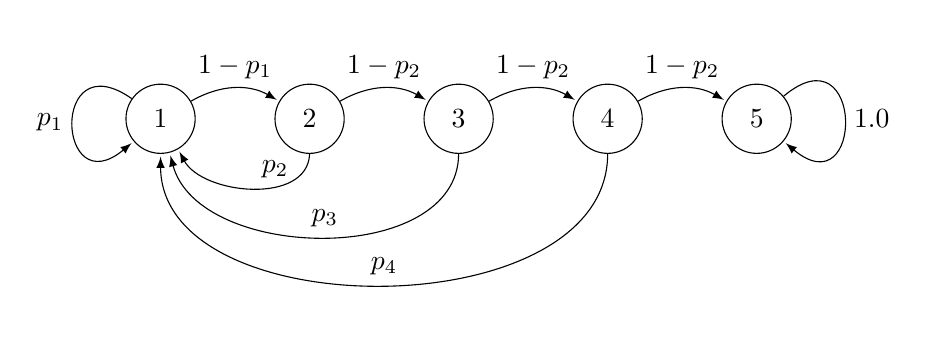
\begin{tikzpicture}[start chain=going right]
    \node[state, on chain]                 (1) {1};
    \node[state, on chain]                 (2) {2};
    \node[state, on chain]                 (3) {3};
    \node[state, on chain]                 (4) {4};
    \node[state, on chain]                 (5) {5};
    \
    \draw[
        >=latex,
    %   every node/.style={above,midway},% either
        auto=right,                      % or
        loop above/.style={out=75,in=105,loop},
        every loop,
        ]
     (1) 	edge[bend left] node [above]{$1 - p_{1}$}   (2)
      		edge[out=145,in=220,loop,looseness=6]             node {$p_{1}$}   (1)
     (2) 	edge[bend left] node[above]{$1 - p_{2}$}   (3)
      		edge[bend left=90,,in=120]             node {$p_{2}$}   (1)
     (3) 	edge[bend left] node[above] {$1 - p_{2}$}   (4)
     		edge[bend left=90,in=105,]             node {$p_{3}$}   (1)
     (4) 	edge[bend left] node [above]{$1 - p_{2}$}   (5)
     		edge[bend left=90,in=90]             node {$p_{4}$}   (1)
     (5) 	edge[out=40, in=320,loop,looseness=6] node[right]{$1.0$}   (5);
    
    
    % The \draw path is like the one above.
    \end{tikzpicture}
    \caption[Markov Chain Model of customer spending]{Markov Chain Model for a particular customer over five periods \parencite[Adapted from Fig. 1]{pfeifer2000modeling}}
    \label{fig:preifermarkovchain}
\end{figure}

% OTHER PREDICTION
Research by Singh et al., from the Massachusetts Institute of Technology, studied the spending behaviour of 52 adults and investigated the impact of social interactions, including text messages, phone calls and face-to-face meetings, on the participants spending in order to predict their spending behaviour. Using a Na\"{i}ve Bayes classifier and selecting a subset of their available features using an Information Gain approach, choosing those with most relevance to each classification task, they were able to correctly classify whether the participant would overspend, explore a diverse range of businesses and remain loyal to a business with 72\% overall accuracy. They concluded that social factors, were better ``predictors of spending behaviour'' than personality traits, which had been previously studied \parencite{singh2013spendingbehaviour}.
%
Although this paper did not study the affects of the participants previous transactions on spending, they were able to predict the users spending behaviour, highlighting that factors other than the transaction history may be of importance when trying to predict a users future outflow. However, the paper does not attempt to make a prediction of the amount spent or how many transactions occur.

% AVERAGES
Smoothing is typically applied to financial market data, for example the value of a particular stock on the FTSE 100. The most common techniques are simple, weighted and exponential moving averages, which all reduce the noise found in the data potentially revealing an orderly process, by removing outliers found in the data. The result of this effect can be seen in Fig \ref{fig:dashweightedaverages} \parencite{dash2012movingaverages}.

\begin{figure}[h]
    \centering
    \includegraphics[width=\textwidth]{background/movingaverages}
    \caption[SMA, WMA and EMA of the S\&P500]{Simple Moving Average (MA) [blue], Weighted MA [red] and Exponential MA [black] of the S\&P500 \protect\footnotemark \parencite[Fig. 5]{dash2012movingaverages}}
    \label{fig:dashweightedaverages}
\end{figure}
\footnotetext{A stock market index of 500 American companies, the US equivalent of the FTSE 500}

These techniques can be applied to a discrete set of numerical time series data, such as personal expenditure over time in order to make an estimate of what the next value in the series will be \parencite{filliben2003nist}. A prediction can be made using the formula in Fig. \ref{fig:weightedmeanforumla}, where $w_{i}$ is the weight and $x_i$ is the value at time period $i$. Simple smoothing is the equivalent of $w_i = 1$, while exponential smoothing is based around a negative exponential law such as $w_i = e^{-n+i}$, both are examples of weighted smoothing and the weights can be decided in different ways depending on what is being predicted. Time periods with a higher weight have a greater affect on the mean, so in order to make a future prediction, the most recent time period would have a higher weight. \question{The chosen implementation details in the design section}

\begin{figure}[h]
    \centering
    \[
        \frac{w_1 x_1 + w_2 x_2 + \cdots + w_n x_n}{w_1 + w_2 + \cdots + w_n}.
    \]
    \caption{Using weighted smoothing to predict a future value}
    \label{fig:weightedmeanforumla}
\end{figure}

% Holt winters extends smoothing, to take into account trends in data
Smoothing (and therefore prediction) can be extended to take into account trends and possible seasonal fluctuations using double and triple smoothing, respectively. A technique known as `Holt-Winters double exponential smoothing` takes into account trends in data, which single smoothing does perform accurately with, by factoring the weighted average growth between previous the time series when calculating the average for each period \parencite{kalekar2004holtwinters}. \question{A demonstration of this is in chapter X?}
% 
Extending the calculation into double and triple smoothing when estimating a users future outflow was decided as a possible extension for the project. \question{Where to mention this?} 

\section{Security}
\question{Should I mention the password entropy paper here? Currently in design}



\chapter{Design}
%\label{cha:part3}

\begin{comment}
Chapter 3: Design
This chapter starts to describe the student's own work. It is where the main design aspects of the project are described. The style of presentation may reflect the life cycle of the project, for example commencing with the Requirements Analysis, but it should not read like a diary. The design should be clearly and precisely described with supporting diagrams. The presentation should be at a fairly high level without excessive detail. This chapter is a suitable place to justify your choice of architecture, implementation technologies and APIs used.
\end{comment}

\plan{This section contains my PLAN of what I will do (before I started) of my app, it should be programming language independent}

This chapter covers design of the system, including an overview of the architecture and descriptions of the key components. 

\section{Statement Management}
The statement management features of the application were selected based on the functionality observed during the background research and conversations with potential users, asking what functionality they would find useful in such an application.

The key features are; parsing of files downloaded from Internet banking, mapping transactions found in the files to real world businesses and 

\subsection{Upload}
\plan{Parsing QIF/OFX, dates being bitches etc...}

\subsection{Named Entity Resolution}

\plan{Must mention what  are}

\subsubsection{Mapping to Entities}
A key part of the project is mapping the text found on a bank statement that represents a business or person to a single entity in the application. After a cleanup of different suffixes that banks append it was found that transactors are often referenced using several names.

Seen in Table \ref{tab:sainsburys}, Sainsbury's was referred to nine different ways in the statement data uploaded by the research participants and similar results are found for most \glspl{transactor}.

\begin{table}[h]
\centering
% SELECT name,count(t.id) as count FROM `transaction` AS t LEFT JOIN global_transactor_mapping AS g ON global_transactor_mapping_id = g.id WHERE global_transactor_mapping_id IN(SELECT id FROM global_transactor_mapping WHERE transactor_id = 7) GROUP BY global_transactor_mapping_id ORDER BY count DESC
\begin{tabular}{@{}ll@{}}
\toprule
Reference            & Occurrences \\ \midrule
sainsburys s/mkts    & 46          \\
sainsburys s/mkt     & 9           \\
sainsburys s/mkts cd & 7           \\
js online grocery    & 2           \\
sainsbury s/mkt      & 2           \\
sainsburys smkt      & 2           \\
js online grocer     & 1           \\
sainsburys superma   & 1           \\
sainsburys-superma   & 1           \\ \bottomrule
\end{tabular}
\caption{References to the same entity `Sainsbury's' found in participant data}
\label{tab:sainsburys}
\end{table}

In consideration of this, the concept of mappings were added to the system. A mapping is a single reference to a transactor, such as `sainsbury s/mkt'. A transactor has multiple mappings. Fig. \ref{fig:mapping} shows this structure.

\begin{figure}[h]
    \centering
    \includegraphics[width=\textwidth]{simple-mappings}
    \caption{Overview of Mappings}
    \label{fig:mapping}
    
    \begin{comment}
%[User]-*<>[Transaction]
[Transaction]<>*-[TransactorMapping]
[TransactorMapping]<>*-[Transactor]
    \end{comment}
\end{figure}


\subsubsection{Global vs User}
Early on it became clear that users should be able to categorise and organise transactions according to their preferences, however categories chosen by a particular user should not affect affect other users.

To support this the application stores two sets of mappings and transactions, User and Global. The structure of the relevant objects is shown in Fig. \ref{fig:transactormappings}. A Transaction can have both a UserMapping and a GlobalMapping, in which case the UserMapping overrides the GlobalMapping when calling methods such as \inlinephp{getMapping()} on the Transaction.

\begin{figure}[h]
    \centering
    \includegraphics[width=\textwidth]{mappings}
    \caption{Overview of User Mappings}
    \label{fig:transactormappings}
    
    \begin{comment}
[Transaction]<>*-0..1[UserMapping]
[Transaction]<>*-0..1-[GlobalMapping]
[User]<>-*[UserMapping]
[UserMapping]<>*-[UserTransactor]
[UserTransactor]<>*-[Category]
[GlobalTransactor]<>*-[Category]
[GlobalMapping]<>*-[GlobalTransactor]
    \end{comment}
\end{figure}



\plan{Use of MySQL to find similar, how that works, alternatives}

\subsection{Suggestions}
\plan{How it uses the above, how the whole user/global thing works}

\section{Prediction}



\subsection{Prediction}
\plan{All the steps that were needed for the prediction}

\subsection{Markov Chain}
\plan{Why I chose first order markov chains, alternatives to that etc...}

\subsection{Weighted Averages}
\plan{How does that work, why is it good?}

\subsection{5 Model System}
\plan{How was is a model chosen for the user?}

\section{Security Considerations}
\todo[inline]{Make this section make sense}
Strong security is of high importance this project, the design considered possible attack vectors and took steps to prevent of reduce the effectiveness of those attacks.

\subsection{Account Hijacking}

Over HTTP information sent between the users web browser and the remote server is sent in plain text. The weakness of this is only enhanced when accessing the internet using an unencrypted wifi connection which would allow anyone in the local area to `sniff' the information sent between the browser and the internet by simply scanning and downloading the packets transmitted.

Although this is a serious security risk this only gets worse when the website involves authentication. Authentication is usually performed by sending the userame and password in plain text to a remote server, which is validated and if correct the user is issued with a session cookie.

A potential attacker could observe and store these usernames and passwords, which is why websites including Facebook used HTTPS for the login, ensuring the usernames and passwords were sent encrypted. 

However, there is still a security flaw if the website falls back to HTTP following the authentication. To prove to the server which website the user represents the user sends their cookie containing a secure ID to the remote server with each request. Although the attacker was unable to sniff the username and password they can perform a session hijack by downloading the content of that cookie to their local machine and prove that they are the user to the remote server accessing all of their data. 
% 
Firesheep was a proof of concept plugin for Firefox released in 2010 that demonstrated this vulnerability, showing that session hijacking could be performed on popular sites including Google, Facebook, Twittter and Flickr, which until recently were not using sidewide SSL.
%http://codebutler.com/firesheep/ FireSheet mention, http://codebutler.github.io/firesheep/

For this reason all of the application uses HTTPS, and redirects users to the HTTPS version if they attempt to access HTTP. This ensured user data is encrypted end to end and cannot be sniffed and neither can their authentication details or session cookie.

\subsection{Password Security}

A common way to crack into user accounts is by brute force. If an attacker knows a particular users username they can perform targeted guessing guessing of the password by enumerating through all possibilities. A websites ability to resist this kind of attack is called the `password guessing resistance'. It is for this reason that many websites, following the guidance of research such as \cite{needed} enforce password rules in an attempt to increase the number of possible combinations for a password, the entropy.

Shannon Entropy can be used estimate the strength of a passwords resistance to this kind of attack. The entropy is calculated using $H(X)= - \sum_{i=1}^n{p(x_i)\log_b p(x_i)}$ where $p(x_i)$ is the probability of the value $x$ occurring \cite{burr2013electronic}.

The paper suggests a predefined set of rules for estimating entropy based on Shannon's work studying English text \cite{burr2013electronic}, however other papers found that using this predefined set of rules was not a valid measure of password strength \cite{weir2010shannon}.
% 
The project uses Shannon's original equation, calculating the probability of guessing an individual character using a formula that takes into account that using a larger character set (such as numbers and symbols) decreases the likely hood of successfully guessing the next character.

As part of a brute force, an attacker may use a dictionary of popular passwords to reduce the testing space before attempting an exhaustion attack. In order to reduce the effectiveness of this kind of attack the project test's any user provided password against a dictionary of at least 50,000 common passwords sourced from password cracking resources \cite{burr2013electronic}.

In addition, to limit the overall effectiveness of brute force attacks, the website rate limits login attempts. If a user attempts to login more than 5 times within one minute, they must wait a minute before they are able to login again.

\subsection{Database Storage}
Unfortunately, it's common for the contents of a websites database to be leaked, whether by an administrator of the website or using other techniques such as SQL injection. It's important to think about the security of the data held within the database, as well as the security of the front end.

pegFinance uses three main techniques to help ensure the security of the users information in the database.

\subsubsection{Passwords}
A users password should never be kept in a reversable state, whether that is plain text\footnote{Unfortunately still very common} or encrypted\footnote{Also common}. If a database of encrypted or plain text passwords is leaked, it is simply a case of finding the encryption key and all the data can be accessed in plain text.

This is why standard security practice is to hash (one-way) passwords. The only way to decrypt a one-way hash is to guess the original input by brute force and see if that matches the output.

However attackers often use of Rainbow tables, collections of precalculated hashes and the input used to create them, allowing an attacker to simply lookup a hash in their database to get the result.

For this reason salting is used, which involves adding a random collection of numbers and letters to each password. This means that the generated hash is dependent on both the users password and the salt and means a Rainbow Table would need to be generated for each user, mitigating the effect.

There is a final step and that's what hashing schema should be used to hash passwords. Traditionally functions such as MD5, SHA1 and SHA256 were used to perform the hashing, however due to advances in modern computer equipment it is possible to generate these at an incredibly fast rate, reducing the time taken to brute force a hash.

Using a deliberately slow hashing function is designed avoid this problem. Blowfish written by Schneier is commonly suggested, as it is designed as a computationally expensive operation. This was demonstrated with a simple test, calculating as many hashes per possible in one second. Table \ref{tab:hashspeed}, shows the results, which found that on average Blowfish took significantly longer to generate each hash.

For this reason the project salts all passwords and hashes them using Blowfish.

\begin{table}[h]
\begin{tabular}{llll}
         & \multicolumn{3}{l}{Hashes Per Second}                   \\
         & Average & Standard Deviation & 95\% Confidence Interval \\
MD5      & \num{2296667} & \num{12923}              & $\pm 8010$                 \\
SHA1     & \num{1869725} & \num{14783}             & $\pm 9162$                 \\
BLOWFISH & 17      & 0                   & $\pm 0$                    \\
\end{tabular}
\label{tab:hashspeed}
\caption{Average number of hashes completed per second on a 2.7Ghz i7 }
\end{table}

\section{Technical Design}

\subsubsection{Personally Identifiable Data}
Of equal concern is other personally identifiable data being leaked, in an attempt to avoid this the application encrypts all information stored in the user table, that is needed at a later date using the AES128 encryption standard. This standard was selected for the project as was endorsed by the U.S. National Institute of Standards and Technology, when outlined by NIST in 2001 and has become the ``encryption standard for commercial transactions in the private sector'' \cite{nist2010aes, stair2009informationsystems}.

\subsubsection{Hashing of Username}
In addition to the above the username of each user is also hashed so it is only known to the person using that account. In the rare case that any of the passwords were brute forced, the relevant username would also need to be brute forced in order to attempt to login or use the details on another website.

\subsection{Other}
Other attack vectors inclung SQL injection and cross-site scripting (XSS) were also considered.

It was decided that the project would use a prepared statements to reduce the risk of SQL injection. By sending the query followed by the parameters as literal values the database server would not interpret them as an executable portion of SQL and attacks, relying on escaping SQL such as \inlinesql$' OR 1$ are prevented.

In order to mitigate the possiblity of XSS the project will need escape all content before displaying it to the user or saving to the database. It was decided that the project would use a templating language that escaped output by default, requiring the output be explicitly marked to avoid escaping. By escaping all content before displaying it to the user a maliciously crafted piece of text such as \inlinehtml$<script>alert(1);</script>$ would be sent to the users browser as \inlinehtml$&lt;script&gt;alert(1);&lt;/script&gt;$ and not interpreted as a script.

\section{Technical Design}

\subsection{Object Orientation}

\subsection{Domain Class}

\subsection{UI Design}

\todo[inline]{Add photos showing the evolution of the UI}



\subsection{Database Class}

\subsection{External Software and Frameworks}
\chapter{Implementation}

\begin{comment}
Chapter 4: Implementation
The implementation details should be confined to the important, difficult or interesting aspects. Large chunks of code should be avoided, and diagrams and tables should be used to present details clearly.
\end{comment}

\plan{Limited to programming languages only}

\section{Security}

\section{Prediction}
\plan{All the steps that were needed for the prediction}

\subsection{Named Entity Resolution}
\plan{Use of MySQL to find similar, how that works, alternatives}

\subsection{Suggestions}
\label{section:suggestion-implementation}
\plan{How it uses the above, how the whole user/global thing works}

\subsection{Markov Chain}
\plan{Why I chose first order markov chains, alternatives to that etc...}

\subsection{Weighted Averages}
\plan{How does that work, why is it good?}

\subsection{5 Model System}
\plan{How was is a model chosen for the user?}

\begin{comment}
Chapter 5: Results
Results that illustrate how the system designed by you works in practice, and how it is intended to be used, may be presented in this chapter. Screen shots may be useful to illustrate how the software interacts with the user.
\end{comment}

\chapter[Results]{Results}

\section{System Walkthrough}
Below, an overview of the systems behaviour is given following the standard users use case in the form of a walk through. For further exploration of features the application can be found online at \url{https://secure.pezcuckow.com/} where an account can be registered for access.

\begin{figure}
\centering
\includegraphics[width=0.8\textwidth]{screenshots/walkthrough/dashboard-empty}
\caption{Empty welcome screen}
\label{fig:welcomescreen}
\end{figure}

Having logged in, the application starts on a welcome screen (Fig. \ref{fig:welcomescreen}) which fills with information over time, for now the system prompts the user to upload a bank statement. The user bar appears at the top of every page\footnote{For clarity both the background and bar are not shown in the following screenshots} which identifies the currently logged in user by name and a avatar pulled using from Gravatar\parencite{gravatar2014avatars}, it provides quick access to the user settings and allows the user to logout.

\begin{figure}
\centering
\includegraphics{screenshots/walkthrough/mainmenu}
\caption{Application main menu}
\label{fig:mainmenu}
\end{figure}

On the left hand side of the screen is the main menu (Fig. \ref{fig:mainmenu}), which is also displayed on all pages. It indicated the currently open page in orange, in theme with the rest of the website, and on hover with a mouse it highlights the chosen page by inverting the colors to make the selection clear.

\subsection{Statement Upload}

\begin{figure}
\centering
\includegraphics[width=0.8\textwidth]{screenshots/walkthrough/upload-empty}
\caption{The upload statement screen before any uploads}
\label{fig:uploadempty}
\end{figure}

Following the advice of the welcome page, the user opens the upload screen (Fig. \ref{fig:uploadempty}). As this is the first time user has opened this screen an information prompt is shown which explains the purpose of the page and reminds them that the files to upload can usually be found on their current banks Internet banking system.

\begin{figure}
\centering
\includegraphics[width=0.8\textwidth]{screenshots/walkthrough/upload-selected}
\caption{UI update following a file selection}
\label{fig:upload-selected}
\end{figure}

After downloading a statement from their, the user uploads the statement by clicks on the select file button and browsing their computer for the file. After confirming their selection the state of the file field changes (Fig. \ref{fig:upload-selected}) to allow checking of the uploaded file and to make it clear one is currently selected. Clicking the primary\footnote{Indicated in orange} upload button uploads the file to the server, which processes it, and refreshes the page.

\begin{figure}
\centering
\includegraphics[width=0.8\textwidth]{screenshots/walkthrough/upload-complete}
\caption{The upload page, following successful file uploads}
\label{fig:upload-complete}
\end{figure}

On the new page (Fig. \ref{fig:upload-complete}), the state of the file upload is indicated above the form, containing a summary of the file uploaded and the uploaded file is highlighted in the recent uploads list, which includes an option to view the transactions uploaded as part of that statement. The highlight color, green, was used to indicate success. 

In addition a further piece of information has been added to the page introduction, the most recent transaction the system knows about is marked in bold, to save the user time when selecting a statement to download.

\begin{figure}
\centering
\includegraphics[width=0.8\textwidth]{screenshots/walkthrough/upload-already}
\caption{Upload confirmation following a duplicate file}
\label{fig:upload-duplicate}
\end{figure}

If the user uploads a file containing no new transactions (all previously uploaded), the confirmation prompt indicates this and it uses the colour yellow to indicate a warning (Fig. \ref{fig:upload-duplicate}).

\begin{figure}
\centering
\includegraphics[width=0.8\textwidth]{screenshots/walkthrough/dashboard-full}
\caption{Welcome screen following statement uploads}
\label{fig:welcome-full}
\end{figure}

\begin{figure}
\centering
\includegraphics[width=0.8\textwidth]{screenshots/walkthrough/piecharthover}
\caption{Additional pie chart detail}
\label{fig:piecharthover}
\end{figure}

On returning to the welcome screen, the dashboard is now full of information\footnote{Fictional information used throughout out this walkthrough} (Fig. \ref{fig:welcome-full}). It provides an overview of the average income and outgoings per month, along with an indication of the users `profit' since the first transaction the application knows about. 

Most notably, the dashboard also includes an interactive pie chart, which gives an indication as to which categories most of their money is spent. On hover the chart gives the actual percentage of the overall expenditure \ref{fig:piecharthover}, and on click opens a page which lists all the transactions in that category.

If the system has suggestions for uncategorised transactors, a notification suggesting they visit the category (or suggestion) wizard is shown.

\section{Suggestion Wizard}
\label{subsection:suggestion-wizard-walkthrough}.

\begin{figure}
\centering
\includegraphics[width=0.8\textwidth]{screenshots/walkthrough/wizard-screen}
\caption{Suggestion wizard main screen, showing suggestions for a reference to Sainsbury's}
\label{fig:wizard-screen}
\end{figure}

The suggestion wizard steps the user though all unmapped and uncategorised references (Fig \ref{fig:wizard-screen}. It starts with the transactor they frequent the most often and prompts them to provide the mapping, either by following a suggestion, creating a new transactor or manually searching for a match.

\begin{figure}
\centering
\includegraphics[width=0.8\textwidth]{implementation/suggestion-notification}
\caption{Notifications shown after completing a sucessfully}
\label{fig:suggestion-complete-notification}
\end{figure}

Completing the mapping, forwards the user to the next unmapped reference, providing confirmation the new mapping has been created as a notification which disappears after a few seconds \ref{suggestion-complete-notification}, and the process repeats.

\begin{figure}
\centering
\includegraphics[width=0.8\textwidth]{screenshots/walkthrough/wizard-create-dropdown}
\caption{Creating a new Transactor and selecting a category}
\label{fig:create-new-transactor}
\end{figure}

\begin{figure}
\centering
\includegraphics[width=0.8\textwidth]{screenshots/walkthrough/wizard-create}
\caption{Selecting a category using the autocomplete feature}
\label{fig:dropdown-autocomplete}
\end{figure}

\begin{figure}
\centering
\includegraphics[width=0.8\textwidth]{screenshots/walkthrough/wizard-map}
\caption{Searching for an existing Transactor using autocomplete}
\label{fig:wizard-map-dropdown}
\end{figure}

The suggestions wizard went through several iterations of user interface enhancements, designed to make it easier to use.
%
For example, when creating a new transactor (Fig. \ref{fig:create-new-transactor}) the system automatically fills in the name field with a pre-formatted version of the reference and the category selection is performed through an upgraded dropdown menu. The dropdown has been upgraded from the standard dropdown found on many websites using client side javascript and provides auto-completion, fuzzy matching, as well as the ability to select a category grouping instead of an exactly category, for example entertainment over Movies \& DVD's (Fig. \ref{fig:dropdown-autocomplete}. A similar dropdown is also used when searching for an existing transactor (Fig. \ref{fig:wizard-map-dropdown}.

After completing the wizard by mapping or ignoring all the unmapped references, the user is congratulated and a hint is given that they should head to the transaction summary page, which includes their monthly expenditure predictions.

\section{Transaction Overview}

\begin{figure}
\centering
\includegraphics[width=0.8\textwidth]{screenshots/walkthrough/transaction-overview}
\caption{The transaction overview screen, which shows expenditure per month and a prediction (in red) for next month}
\label{fig:transaction-overview}
\end{figure}

The transaction overview screen shows spending per month in each of the categories and a the prediction for next month made using the machine learning techniques outlined in \autoref{section:prediction-system} (Fig. \ref{fig:transaction-overview}). At the top of the screen a summary of the total income, expenditure and net profit for each month is shown. The rest of the page is split into two sections, representing money coming into and leaving the users account. In the example shown the user hasn't mapped all of their references and so some transactions are listed under uncategorised, a hint is placed at the top of the screen reminder users to visit the category wizard. 

\begin{figure}
\centering
\includegraphics[width=0.8\textwidth]{screenshots/walkthrough/transaction-subcategories}
\caption{The subcategories being used to make up a category in the overview}
\label{fig:transaction-subcategories}
\end{figure}
.png

Clicking on any of the rows in the table reveals the subcategories and their associated values that are being used to produce the row, using an animated `slide-down' effect \ref{fig:transaction-subcategories}. 

\section{Viewing Statements}
\begin{figure}
\centering
\includegraphics[width=0.8\textwidth]{screenshots/walkthrough/statement-view}
\caption{The statement view}
\label{fig:statement-view}
\end{figure}

\begin{figure}
\centering
\includegraphics[width=0.8\textwidth]{screenshots/walkthrough/statements-group-category}
\caption{Grouping the statement by category}
\label{fig:statements-group-category}
\end{figure}

\begin{figure}
\centering
\includegraphics[width=0.8\textwidth]{screenshots/walkthrough/statements-groupby-company}
\caption{Grouping the statement by category}
\label{fig:statements-groupby-company}
\end{figure}

The application also provides an easy way to view historical spending organised by month (Fig \ref{fig:statement-view}). The transactions in each month can be grouped by category, transactor or date to give a more detailed idea of how money is being spent (Figs. \ref{fig:statements-group-category} and \ref{fig:statements-groupby-company}).

\begin{figure}
\centering
\includegraphics[width=0.8\textwidth]{screenshots/walkthrough/view-reference}
\caption{Recent transactions at a particular transactor}
\label{fig:view-reference}
\end{figure}

\begin{figure}
\centering
\includegraphics[width=0.8\textwidth]{screenshots/walkthrough/view-reference-unmapped}
\caption{Viewing an unmapped reference}
\label{fig:view-reference-unmapped}
\end{figure}

A user can also view particular transactor or reference, which includes the references category and a summary of recent transactions (Fig. \ref{fig:view-reference}). If the reference is not yet mapped, options similar to those shown in the suggestions wizard are listed enabling them to map the reference correctly (Fig. \ref{fig:view-reference-unmapped}). 

\section[Responsive Design]{Responsive Web Design}
A key feature of the application is being able to access it at any time from any device, particularly when taking into account the rapid increase in the use of mobile devices.  Interacting with a website on a smartphone or tablet is not the same as interacting using a computer, due to the smaller screen size and use of touch over a mouse.

Forbes reported that 24\% of their 2013 website visits came from mobiles and 13\% from tablets, down from a total of 15\% in 2012. particularly with the high percentage of website visits coming from mobile devices \parencite{steimle2013responsive}.

In order to ensure the project is accessible from a variety of different devices the core UI uses Responsive Web Design (RWD) to layout the website differently depending on the screen size of the device to ensure an optimal viewing experience.

The differences depending on the device are highlighted in Figs. \ref{fig:responsive-macbook}-\ref{fig:responsive-iphone}.

\begin{figure}[h]
    \centering
    \includegraphics[width=0.8\textwidth]{screenshots/responsive/macbook}
    \caption{Layout on a standard laptop}
    \label{fig:responsive-macbook}
\end{figure}

\begin{figure}[h]
    \centering
    \includegraphics[width=0.8\textwidth]{screenshots/responsive/ipad-sideways}
    \caption{Layout on a tablet in landscape}
    \label{fig:responsive-ipad}
\end{figure}

\begin{figure}
\centering
\begin{minipage}{.5\textwidth}
    \centering
    \includegraphics[width=0.45\textwidth]{screenshots/responsive/ipad-portrait}
    \captionof{figure}{Layout on a tablet in portrait}
    \label{fig:responsive-ipad2}
\end{minipage}%
\begin{minipage}{.5\textwidth}
    \centering
    \includegraphics[width=0.5\textwidth]{screenshots/responsive/iphone-portrait}
    \captionof{figure}{Layout on a smaller smartphone}
    \label{fig:responsive-iphone}
\end{minipage}
\end{figure}

%\section{Uploading a Statement}

%\section{Suggestion Engine}

%\section{Viewing Statements}

%\section{Prediction Overview}
%\chapter{Testing and Evaluation}
\label{cha:testing}

\begin{comment}
Chapter 6: Testing and Evaluation
This chapter should give details of how the system designed and implemented by you was tested. The data and results obtained from this testing whould be presented and consideration be given as to whether or not these results confirm that everything works correctly.

The analysis of test results is very important and some assessment of their significance and quality must be given. Likely sources of error and inaccuracy should be mentioned. Use graphs, bar charts and histograms where appropriate, remembering to label all axes and give scales. The analysis is often done badly, thus sacrificing marks.
\end{comment}

The evaluation of the application indicates that these three objectives have been met. Preliminary research demonstrates that enjoyed using the application and that the majority of participants would use it in the future if implemented as a full product. Testing with participant data shows that the average absolute error of the prediction engine was $PERCENTAGE\%$ for users with over three months historical information. Preliminary penetration testing, using both white-box and black-box testing indicated that the security protections put in place are effective.  However, the evaluation of the project was limited, due to the size of the user base, discussed further in \autoref{sec:limitations}. \todo{Complete this}

\section{During Development}
Though-out the development of the project, predominantly after each feature was implemented and before a new iteration was started the applications functionality was tested through face to face conversations, observations and unit testing.

\subsection{Acceptance Testing}
As noted throughout the report, the application was regularly tested by potential end users and the developers during lab observations where the user was asked to complete a task on the website while describing what they were doing. 

During the testing, common pain points were identified and these were used to decide on the future features, either to improve the user experience on the website, making it easier to use, or to support a new use case.

Example modifications, made as a result of these observations, include the dropdown menu autocompletion when creating and mapping transactors, the hints that appear throughout the website to guide the user onto the next task, and the suggestion wizard.

Towards the beginning of the project these meetings were used to evaluate and update the design of the user interface, which went through several different designs, and to receive qualitative feedback from the users (Fig. \ref{fig:ui-design}).

\begin{figure}
\centering
\begin{subfigure}{0.34\textwidth}
  \centering
  \includegraphics[width=0.95\linewidth]{testing/uidesign1}
\end{subfigure}%
\begin{subfigure}{0.34\textwidth}
  \centering
  \includegraphics[width=0.95\linewidth]{testing/uidesign2}
\end{subfigure}
\begin{subfigure}{0.31\textwidth}
  \centering
  \includegraphics[width=0.95\linewidth]{testing/uidesign3}
\end{subfigure}
\caption{A few iterations of the user interface designs}
\label{fig:ui-design}
\end{figure}

\subsection{Unit Testing}
High risk classes, including the Budget, the QIF and OFX Parsers implementing the TransactionFileParserInterface, and those implementing the TransactionCollectionInterface were unit tested to ensure the functionality of the classes was not affected when implementing new features or refactoring the code.

These classes were selected as the core functionality of the application relied on their behaviour and they were coupled to the most other classes, for example the Budget object was responsible for holding a collection of Transactons in the tree data structure described in \autoref{section:prediction-implementation} and performed the majority of the prediction functionality, holding references to the TransactionMarkovChain, TransactionWeightedAverageCalculator and PredictionEvaluation.

Due to time constraints and the complications of testing data driven classes, both the number of unit tested classes and methods covered was limited, this is discussed further in \autoref{sec:limitations}.

\section{After Development}
Once development of the project was halted the application was tested in the three following the three sections outlined through the report. The statement management functionality was assessed using a questionnaire posed to research participants that were given access to the system, the prediction algorithms were evaluated using the sample data provided by the research participants and the security of the application was evaluated using penetration testing.
%
Unfortunately the reliability of the results for both the statement management and prediction is questionable due to the limited number of research participants and questionnaire responses, see \autoref{sec:limitations}.

% This chapter should give details of how the system designed and implemented by you was tested. The data and results obtained from this testing whould be presented and consideration be given as to whether or not these results confirm that everything works correctly.
% The analysis of test results is very important and some assessment of their significance and quality must be given. Likely sources of error and inaccuracy should be mentioned. Use graphs, bar charts and histograms where appropriate, remembering to label all axes and give scales. The analysis is often done badly, thus sacrificing marks.

\subsection{Statement Management}
The questionnaire posed to the research participants was split into three sections, a full copy of the questions can be found in Appendix \ref{app:questionnaire}.

The first made a series of statements and asked the respondent to answer on a five point scale, ranging from 1, strongly disagree to 5, strongly agree. The questions in this sections had four main types, and were selected following the structure of the Standardized Universal Percentile Rank-Questionnaire \ref{sauro2011standardized} which is used by companies including PayPal to assess their websites. 
%
Questions on usability focused on how easy users found navigation of the website, locating the information they needed, and whether they enjoyed using it.
%
Credibility questions focused on whether the user trusted the website having uploaded their personal information.
%
The likely hood of a user recommending the site to their colleagues and friends or returning to the site in the future gave an idea of the potential loyalty the participants expressed.
%
The last focused on the user interface to gain an idea of whether the website appealed to the users.

The second section focused on task completion, participants were asked to complete a task and then rate the how difficult or easy they found that on a seven point scale.
%
This section was designed to assess the functionality of the website and to identify additional pain points.
%
One scale question was asked per task as research suggests that use of a single question performs just as well as breaking the task down into sub-questions \parencite{sauro2009comparison, sauro2009correlations}, however a free text field was included with each task to obtain qualitative information on the reasons behind the answer.

In final section was used to identify features of the the website that users favoured and to allow for feature requests, all questions were answered in free text fields

The average respondant said the website was easy to nativate, 3.80.

Comfortable using the website: 3.80

Completed visit 4.20
Reccoment website if complete 4.00

Attractive 3.80

Downloading from bank 5.40
Upload statement 6.80
View statement 6.00
Prediction 4.40
Overall use: 5.60

\subsection{Prediction}

\subsection{Security}

% The evaluation of the application indicates that these three objectives have been met. Preliminary research demonstrates that enjoyed using the application and that the majority of participants would use it in the future if implemented as a full product. Testing with participant data shows that the average absolute error of the prediction engine was $PERCENTAGE\%$ for users with over three months historical information. Preliminary penetration testing, using both white-box and black-box testing indicated that the security protections put in place are effective.  However, the evaluation of the project was limited, due to the size of the user base, discussed further in \autoref{sec:limitations}. \todo{Complete this}

\plan{How did I check that it was working? Testing with personal data, users trying it and running tests of everything}

\missingfigure{Need figures representing accuracy, error, etc}

\section{User feedback}

% SUPR-Q - http://www.measuringusability.com/suprq.php


\plan{User surveys to check what they wanted}

\chapter{Conclusions}

\begin{comment}
Chapter 7: Conclusions
This can be a short chapter summarizing what you have achieved and what you have learned from the achievement. It is different from the abstract. The main results of your work should be highlighted with a critical appraisal of them indicating the extent to which the objectives outlined in Chapter 1 have been met. Exaggerated claims are counterproductive here. Recommendations for further activity are often included in this chapter.
\end{comment}

\section{Key Things Learnt}
\plan{How to do prediction, password entropy, other stuff}

\section{Does the system do what I set out to do?}
\plan{Does it make accurate predictions (summarise the evaluation section)}

\section{Further research}
\plan{Would like to classify users, would like to take into account global spending patterns}
% Gamification, global patterns

\subsection{Overfitting models}
\label{section:overfittingmodels}

\plan{Include why having too many models is bad and explore those a bit}

\subsection{Using Learning to Select a Scaling Parameter}
\label{section:learningscalingparameter}

\plan{How learning algorithms could be used to fit the weights even more (custom one for each user!)}

\section{Limitations of research?}
\plan{Limited set of testers, just students and friends, add more stuff and then go global.}



%% References
% There are a number of schemes for presenting references to the reader. Most publications are very strict about their presentation and, unfortunately, there is no unanimity of format across the range of relevant publications. The recommended method, used in IET and IEEE journals, is to identify each reference with a number located at the appropriate point of the text in square brackets, e.g. [42]. This is the recommended format for project reports in Computer Science. The list of references included in your report must give all the relevant information to enable the reader to find it.

% references
\printbibliography

% appendix
\begin{appendices}

\chapter{Survey} \label{app:budgetsurvey}
Informal survey of 12 CS students in the third year lab. 

Questions:
\begin{enumerate}
\item Do you currently make a budget?
\item Do you stick to that budget?
\item Do you find your budget has a `positive' impact?
\end{enumerate}

% Booktabs require to add  to your document preamble
\begin{table}[h]
\centering
\caption{Survey Results}
\begin{tabular}{@{}llll@{}}
\toprule
       & \multicolumn{3}{l}{Question} \\ 
Answer & 1.       & 2.      & 3.      \\ \midrule
yes    & 5        & 1       & 3       \\
no     & 7        & 4       & 4       \\
n/a    & 0        & 7       & 5       \\ \bottomrule
\end{tabular}
\end{table}

\begin{comment}
Appendix A, B, C, etc.
These appendices can be very useful for giving detail that would otherwise disrupt the flow and readability of the report. They are given titles (e.g. "Appendix A: Example of the operation of the system") and bound in with the report. In general they are optional though, by convention, for a programming project, Appendix A often contains a non-trivial illustrative example of an input to the system and the corresponding output. For some projects, appendices may include tables of data. However, very long tables of data (more than about 10 pages) should be relegated to the Auxiliary Material, and not submitted as part of the Final Report. Program listings (apart from short code snippets) should likewise not be submitted as part of the Final Report.
\end{comment}

\chapter{Hashing Test} \label{app:hashingtest}

Implemented in PHP, test was run on a 2.7 Ghz Intel Core i7 with 16Gb of 1600Mhz DDR3 RAM.

\lstinputlisting[style=phpcolor]{code/passwordHashingTest.php}

\chapter{External Libraries} \label{app:externallibraries}

A full list of libraries and frameworks used by pegFinance.

\section{Back End}
\textbf{pegFramework}
MVC framework that pegFinance is based around. 

Licence - self developed, open-source under the MIT license

\textbf{Propel}
ORM library for PHP, that converts schemas based in XML into PHP objects and provides database connectivity.
%
The database objects found within pegFinance are defined in, and generated by Propel. 

License - open-source project released under the MIT license

\textbf{Less}
CSS pre-processor that extends the CSS, adding additional features and functionality. `.Less` files compile to `.css`.
%
The CSS for pegFinance is written in and compiled with Less.

License - Apache 2 License

\section{Front End}
\textbf{jQuery}
A `feature-rich JavaScript library', that provides element selection and enabled HTML traversal and manipulation, as well as providing an easy API for Ajax requests.
%
Used throughout the site for frontend effects, and used heavily in the suggestion wizard.

License - open-source, released under the MIT license

\textbf{Bootstrap}
Front-end framework for faster web development that provides a large collection of predefined CSS classes and elements for use on the page.
%
Used for the UI of pegFinance.

License - MIT license and is copyright 2014 Twitter

\textbf{Inspiritas}
A theme for bootstrap, that defines colors and additional elements for use on the page.
%
A heavily modified version is used for the UI of pegFinance.

Licence - Open-source, Apache License

\textbf{StrongPass.js}
jQuery Password Strength plugin for Twitter Bootstrap.
%
Modified version used to provide a client side indication the password entropy calculation during signup.

License - Dual, under the MIT and GPL.

\textbf{Pines Notify}
jQuery Pines Notify Plugin. Used to provide event notification in the user interface to indicate events.
%
pNotify is used in the suggestion wizard and when mapping a reference to a transactor to update the user on the status of the request

Licence - Triple license under the GPL, LGPL, and MPL.

\textbf{UserVoice JavaScript SDK}
SDK for access to a user opinion platform, to help provide insight into the userbase and receive feedback.
%
Deployed throughout the application so users can provide feedback when using the application, including an optional screen capture.

Licence - Commercial SDK provided by UserVoice

\textbf{Chosen}
Javascript library used to make `long, unwieldy select boxes much more user-friendly'.
%
Used to improve user experience when categorising transactors, including search.

Licence - MIT license

\textbf{Highcharts}
Highcharts is a charting library written in HTML5/JavaScript.
%
It's used to draw the pie charts on the home page and charts throguhout the application.

Licence - Creative Commons Attribution-NonCommercial 3.0 License.

\textbf{Base Admin}
Admin theme, used on the non user facing admin pages.

License - Commercial Single Use license

\chapter{PHP Code} \todo{Needs a better name}

\begin{figure}
\lstinputlisting[style=phpcolor]{code/setTransactorMethod.php}
\caption{PHP Transaction->setTransactor(\$name) method source code}
\label{fig:settransactor}
\end{figure}

\begin{figure}
\lstset{style=phpcolor}
\begin{lstlisting}
if($dmy && $mdy || !$dmy && !$mdy)
    // ... prompt the user
else
    // ... continue conversion using the detected month format
\end{lstlisting}
\caption{Whether or not to prompt the user following month format detection}
\end{figure}
\chapter{Suggestion Wizard JSON}

The suggestion wizard is powered by AJAX, which makes JSON requests to a RESTful API on the backend, Fig. \ref{fig:json-examples} outlines an example set of communication.

\begin{figure}
    \begin{subfigure}[a]{\textwidth}
        \lstinputlisting[language=json]{code/suggestions.json}
        \caption{GET request sent \lstinline{/ajax/transactor/suggestions}}
    \end{subfigure}
    
    \begin{subfigure}[b]{\textwidth}
        \lstinputlisting[language=json]{code/map.json}
        \caption{POST request sent to \lstinline{/ajax/transactor/map}}
    \end{subfigure}
\end{figure}

\begin{figure}
    \ContinuedFloat   
    \begin{subfigure}[c]{\textwidth}
        \lstinputlisting[language=json]{code/create.json}
        \caption{POST request sent to \lstinline{/ajax/transactor/create}}
    \end{subfigure}
    
    \begin{subfigure}[d]{\textwidth}
        \lstinputlisting[language=json]{code/reply.json}
        \caption{Response from API following a successful map or create}
    \end{subfigure}    

    \caption{JSON encoded requests to the RESTful API}
    \label{fig:json-examples}
\end{figure}

\end{appendices}

\end{document}
